\documentclass[border=9pt]{standalone}
\usepackage[fontset=fandol]{ctex}
\usepackage{amsmath,amssymb,tikz}
\usetikzlibrary{arrows.meta,calc,decorations.pathmorphing}
\tikzset{arr/.style={-{Stealth[length=2mm]},semithick}}
\begin{document}

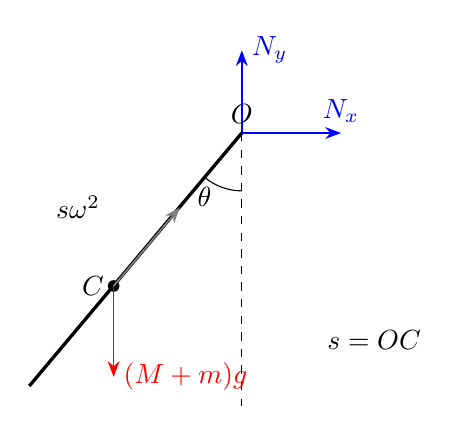
\begin{tikzpicture}[scale=1.05]
\coordinate(C)at(-1.55,-1.85); \draw[very thick](0,0)--(-2.57,-3.06);
\node[above]at(0,0){$O$};\fill(C)circle(2pt)node[left]{$C$};
\draw[dashed](0,0)--(0,-3.3);\draw (0,-.7) arc(-90:-130:.7)node[below]{$\theta$};
\draw[arr,blue](0,0)--(1.2,0)node[above]{$N_x$};
\draw[arr,blue](0,0)--(0,1)node[right]{$N_y$};
\draw[arr,red](C)--++(0,-1.1)node[right]{$(M+m)g$};
\draw[arr,gray](C)--++(.8,.95);\node[left]at(-1.6,-.9){$s\omega^2$};
\node at(1.6,-2.5){$s=OC$};
\end{tikzpicture}
\end{document}
